\documentclass[11pt,a4paper]{article}

\usepackage[utf8]{inputenc}
\usepackage[T1]{fontenc}
\usepackage[italian]{babel}
\usepackage{amsmath, amssymb}
\usepackage{geometry}
\usepackage{booktabs}
\usepackage{array}
\usepackage{graphicx}
\usepackage{hyperref}
\usepackage{xcolor}
\usepackage{enumitem}
\usepackage{caption}

\geometry{margin=2.5cm}
\hypersetup{colorlinks=true, linkcolor=blue, urlcolor=blue}

\title{Da PCA a PCR a PLS:\\
  un'estensione del benchmark lineare IFC tramite riduzione di dimensionalità}
\author{Progetto di Statistica Applicata --- Report di estensione PCR}
\date{}

\begin{document}
\maketitle

\begin{abstract}
\noindent
Questo report risponde a un'osservazione specifica del docente
(\emph{``PCR non PCA?''}) estendendo l'analisi descrittiva delle
componenti principali del progetto (script 02 / 02b / 02c) in una
Principal Component Regression a fini predittivi. Il lavoro è
organizzato in tre passi. Primo: applichiamo la PCR ai
\(326\) predittori GRINS V3 ingegnerizzati usati dal benchmark
LASSO e dal modello parsimonioso. Secondo: applichiamo la PCR ai
\(12\) indicatori IFC che costituiscono l'indice stesso, in un
esercizio volutamente quasi tautologico che usiamo come controllo
di sanità sulla costruzione dell'IFC. La presenza di un residuo
irriducibile di \(\sim 1{,}3\%\) rivela che l'IFC raw \emph{non} è
una combinazione lineare pura dei dodici indicatori; lo scarto è
coerente con il passaggio standard di rango percentuale che la
metodologia ufficiale applica prima dell'aggregazione pesata.
Terzo: aggiungiamo le Partial Least Squares (PLS) come naturale
competitor information-aware della PCR. La PLS domina la PCR di
circa cinque punti percentuali di \(R^{2}\) a ogni \(K\), e pareggia
il benchmark LASSO a \(K = 75\) senza mai offrirne
l'interpretabilità. La conclusione è che LASSO resta il metodo
preferito per questo problema, ma la PLS è un upper bound
non-interpretabile difendibile; la PCR da sola è subottimale perché
la direzione predittiva nei nostri dati non coincide con la
direzione di massima varianza.
\end{abstract}

\section{Perché è stata aggiunta un'estensione PCR}

La cascata descrittiva di PCA del progetto (script
\texttt{02\_pca.R}, \texttt{02b\_pca\_all.R},
\texttt{02c\_pca\_presentation.R}) decompone i \(12\) indicatori
IFC in componenti principali e caratterizza come la loro varianza
si distribuisce tra anni e tra indicatori. Non utilizza, però, le
componenti risultanti per fare predizione. Il docente ha fatto
notare che l'estensione naturale di quell'analisi descrittiva è
una Principal Component Regression: \emph{usare le PC come
regressori in un modello per l'IFC}.

Questo è metodologicamente diverso dal benchmark LASSO e dal
modello parsimonioso documentati in
\verb|reports/parsimonious_extension|. Quei due approcci
costruiscono un modello sulle \emph{variabili originali} GRINS,
dopo o penalizzazione \(\ell_{1}\) o pruning VIF + ranking +
filtro di significatività. La PCR sostituisce l'intero passo di
selezione con una \emph{riduzione di dimensionalità}: prende un
piccolo insieme di nuove variabili (le PC), definite come
combinazioni lineari di \emph{tutte} le originali, e regredisce
il target su di esse.

Le domande a cui vogliamo rispondere sono:
\begin{itemize}[leftmargin=2em]
  \item Come si comporta la PCR sulle stesse \(326\) features
    GRINS, out-of-sample, rispetto al benchmark LASSO e al modello
    parsimonioso?
  \item La PCR applicata direttamente ai \(12\) indicatori IFC
    riproduce l'IFC, e se no, cosa rivela il residuo?
  \item La sottoperformance della PCR, quando si verifica, è una
    proprietà del metodo o dei nostri dati? La PLS risolve la
    questione.
\end{itemize}

\section{Metodo}

\subsection{Notazione e cross-validation panel-aware}

In tutto il report, \(\mathbf{X}\in\mathbb{R}^{n\times p}\) è la
matrice dei predittori standardizzati, \(\mathbf{y}\in\mathbb{R}^{n}\)
è il target IFC, \(n = 15\,782\) è il numero di osservazioni
comune--anno, e \(K\) è il numero di componenti trattenute. Tutte
le metriche di performance usano la stessa
\textbf{cross-validation panel-aware a 5 fold} del resto del
progetto: ogni comune (sia le righe del \(2019\) sia quelle del
\(2021\)) sta in un singolo fold, così il set di test contiene
sempre comuni che il modello non ha mai visto. Riportiamo media e
deviazione standard di \(R^{2}\) tra i fold.

Un indicatore binario \(\mathrm{year2021}_i\in\{0,1\}\) è incluso
come effetto fisso separato in ogni regressione ma è escluso dalla
costruzione delle componenti principali / PLS, perché una
variabile binaria distorce le direzioni principali ed è
concettualmente un controllo, non contenuto.

\subsection{Principal Component Regression}

La PCR procede in due passi. Primo, la matrice di covarianza
campionaria di \(\mathbf{X}\) viene diagonalizzata:
\begin{equation}
  \tfrac{1}{n}\,\mathbf{X}^{\top}\mathbf{X}
  \;=\;
  \mathbf{V}\,\Lambda\,\mathbf{V}^{\top},
  \qquad
  \mathbf{Z} \;=\; \mathbf{X}\,\mathbf{V}.
  \label{eq:pca}
\end{equation}
Le colonne di \(\mathbf{V}\) sono le direzioni principali; le
colonne di \(\mathbf{Z}\) sono gli score delle componenti
principali. Gli autovalori in \(\Lambda\) sono ordinati in modo
decrescente, quindi la componente \(j\) porta la \(j\)-esima quota
più alta di varianza totale in~\(\mathbf{X}\). Secondo: una
regressione lineare di \(y\) sulle prime \(K\) componenti più il
fixed effect anno viene fittata con OLS:
\begin{equation}
  \widehat{\mathrm{IFC}}_i
  \;=\;
  \beta_{0}
  + \sum_{j=1}^{K} \beta_{j}\,Z_{ij}
  + \gamma\,\mathrm{year2021}_{i}.
  \label{eq:pcr}
\end{equation}
La proprietà cruciale di \eqref{eq:pca} è che essa
\emph{ignora}~\(y\): le direzioni principali sono quelle di
massima varianza in~\(\mathbf{X}\), non quelle di massimo
contenuto predittivo per~\(y\). La PCR funziona bene solo quando
le due direzioni coincidono.

\subsection{Partial Least Squares}

La PLS è l'analogo predittivo naturale della PCR: sceglie lo
stesso tipo di componenti ma usando \(y\) a ogni passo. La
componente \(j\) è definita come la combinazione lineare di
\(\mathbf{X}\) che massimizza la covarianza campionaria con il
(residuo di) \(y\) date le componenti precedenti. Formalmente, la
prima direzione PLS risolve
\begin{equation}
  \mathbf{w}_{1}
  \;=\;
  \arg\max_{\|\mathbf{w}\| = 1}
    \mathrm{Cov}\!\left(\mathbf{X}\mathbf{w},\,\mathbf{y}\right),
  \label{eq:pls1}
\end{equation}
e le direzioni successive iterano dopo aver deflattato sia
\(\mathbf{X}\) sia \(\mathbf{y}\) della varianza già catturata.
Usiamo \texttt{pls::plsr} e aggiungiamo il fixed effect anno alla
predizione finale come per la PCR.

\subsection{Tre pipeline concrete}

Eseguiamo tre analisi concrete:
\begin{itemize}[leftmargin=2em]
  \item \textbf{Script 18 (PCR su GRINS V3).} \(\mathbf{X}\) è la
    matrice GRINS ingegnerizzata da 326 feature, la stessa usata
    dal benchmark LASSO.
  \item \textbf{Script 18b (PCR sui 12 indicatori IFC).}
    \(\mathbf{X}\) è la matrice 12-indicatori da cui l'IFC
    ufficiale è costruito. Vengono applicati gli stessi flip di
    polarità dello script 02. Il target è il valore IFC raw.
  \item \textbf{Script 18c (PLS vs PCR su GRINS V3).} Sia PCR sia
    PLS vengono fittate sulla stessa matrice GRINS ingegnerizzata
    dello script 18 e confrontate agli stessi valori di \(K\).
\end{itemize}

\section{Risultati}

\subsection{PCR su GRINS V3: la riduzione di dimensionalità è subottimale}

La Figura~\ref{fig:scree_grins} mostra lo scree plot della PCA
sulle \(326\) feature ingegnerizzate. La varianza è distribuita su
molte componenti: ne servono 50 per raggiungere il \(\sim 60\%\)
del totale, e 100 per circa l'80\%.

\begin{figure}[h!]
  \centering
  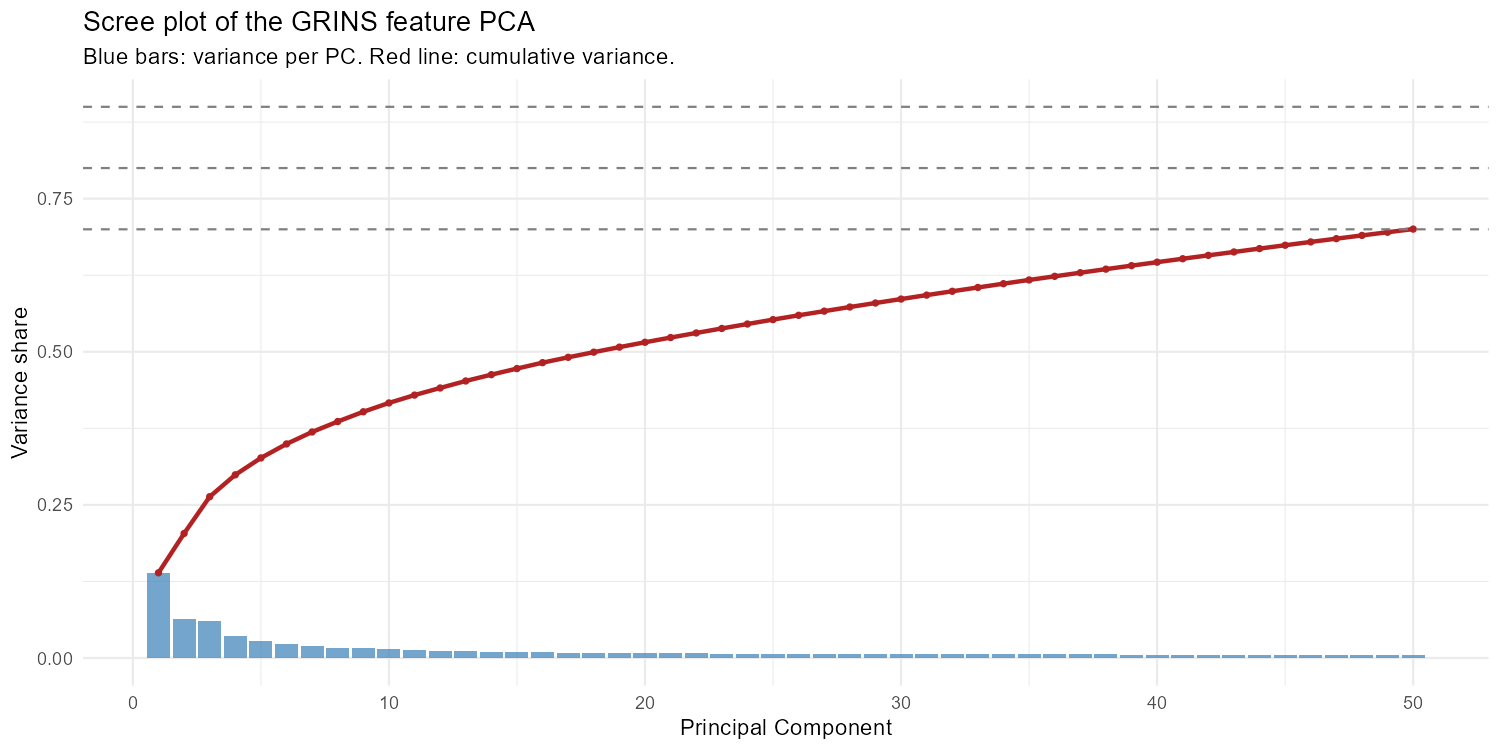
\includegraphics[width=0.85\textwidth]{figures/scree_grins.png}
  \caption{Scree plot della PCA sulla matrice GRINS V3
    ingegnerizzata (prime 50 PC). Barre blu: varianza marginale
    per PC. Linea rossa: varianza cumulata.}
  \label{fig:scree_grins}
\end{figure}

La Tabella~\ref{tab:pcr_grins} e la Figura~\ref{fig:trade_grins}
riportano l'\(R^{2}\) out-of-sample della PCR in funzione di
\(K\). Le linee tratteggiate orizzontali segnano il benchmark
LASSO (\(R^{2} = 0{,}825\)) e il modello lineare parsimonioso
(\(R^{2} = 0{,}784\)).

\begin{table}[h!]
  \centering
  \begin{tabular}{ccccc}
    \toprule
    \(K\) & \(R^{2}\) & RMSE & MAE & varianza cumulata \\
    \midrule
    5    & 0,69 (approssimato) & 2,32 & 1,77 & 12\,\% \\
    25   & 0,771 & 2,00 & 1,50 & 28\,\% \\
    50   & 0,778 & 1,96 & 1,48 & 41\,\% \\
    75   & 0,779 & 1,96 & 1,47 & 50\,\% \\
    100  & \textbf{0,787} & \textbf{1,92} & \textbf{1,45} & 59\,\% \\
    \bottomrule
  \end{tabular}
  \caption{PCR sulla matrice GRINS a 326 feature, CV panel-aware
    a 5 fold. Anche con cento componenti principali, la PCR resta
    sotto il modello lineare parsimonioso (che usa solo 25
    variabili originali) e quattro punti di \(R^{2}\) sotto il
    benchmark LASSO.}
  \label{tab:pcr_grins}
\end{table}

\begin{figure}[h!]
  \centering
  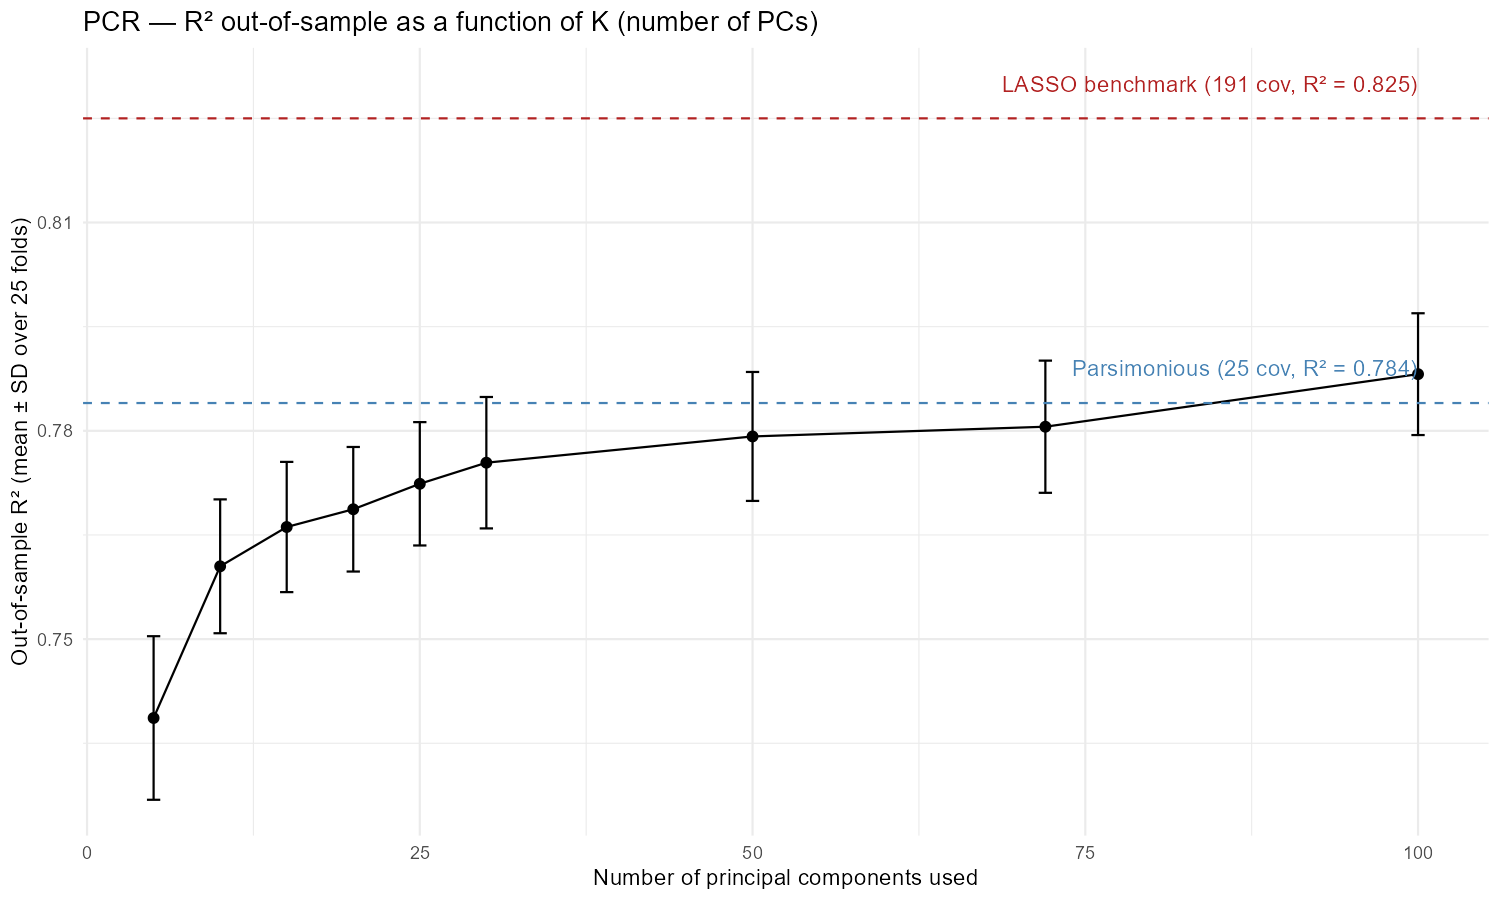
\includegraphics[width=0.85\textwidth]{figures/tradeoff_grins.png}
  \caption{Curva di trade-off PCR sulle feature GRINS V3.
    \(R^{2}\) medio out-of-sample su 25 fold di CV panel-aware,
    con barre d'errore di \(\pm 1\) deviazione standard. La PCR
    ha bisogno di circa 100 PC per raggiungere
    \(R^{2} \approx 0{,}787\), ancora sotto il LM parsimonioso (25
    variabili, \(R^{2} = 0{,}784\)) e quattro punti sotto il
    benchmark LASSO (191 variabili, \(R^{2} = 0{,}825\)).}
  \label{fig:trade_grins}
\end{figure}

\paragraph{Due letture dello stesso grafico.}
Primo: su base assoluta, la PCR non riesce a pareggiare il
benchmark LASSO nemmeno con cinque volte tante componenti: 100 PC
raggiungono \(0{,}787\), ancora \(-0{,}038\) sotto il LASSO a
\(0{,}825\). Secondo: su base \emph{per-componente}, la PCR è
ancora meno efficiente di quanto il conteggio ingenuo suggerisca.
A \(K = 25\) la PCR fa \(0{,}772\), circa \(1{,}3\) punti
percentuali sotto il modello lineare parsimonioso sullo stesso
numero di variabili originali. È la firma empirica del
\emph{disallineamento tra varianza e predizione}: le direzioni
principali di \(\mathbf{X}\) non sono le direzioni in cui vive il
segnale IFC.

\subsection{PCR sui 12 indicatori IFC: un controllo quasi tautologico}

Gli script in cascata \texttt{02\_pca.R / 02b / 02c} calcolano la
PCA descrittiva sui 12 indicatori IFC
\(\mathrm{Ind1},\dots,\mathrm{Ind12}\). La controparte predittiva
naturale è regredire l'IFC raw sulle PC principali di quegli
stessi dodici indicatori. Poiché l'IFC è costruito, almeno
nominalmente, per aggregazione di quelle stesse dodici variabili,
l'esercizio è prossimo alla tautologia: una regressione su tutti i
dodici indicatori originali dovrebbe riprodurre l'IFC quasi
esattamente.

\paragraph{Una scoperta sui dati.}
La prima esecuzione di questo script ha restituito un
\(R^{2} = 0{,}982\) apparentemente incompleto. Indagando abbiamo
scoperto che il file
\texttt{IFC\_Final\_Analysis\_Sorted.xlsx} contiene un piccolo
numero di voci \(\mathrm{PRO\_COM} \times \mathrm{year}\)
duplicate con valori IFC incoerenti (es.\ il comune 5122 nel 2021
compare due volte con IFC = 100 e IFC = 110 rispettivamente). La
pipeline basata su GRINS maschera il problema implicitamente
tramite un inner join con un pannello GRINS univoco; qui, con solo
i 12 indicatori dal lato dei predittori, i duplicati emergono.
Abbiamo aggiunto un passo \verb|distinct(PRO_COM, year)| su
entrambi i lati del merge prima di rieseguire.

\paragraph{Il restante \(1{,}3\%\) è informativo.}
Dopo la deduplica la PCR con \(K = 12\) raggiunge
\(R^{2} = 0{,}987\), vedi Tabella~\ref{tab:pcr_ifc} e
Figura~\ref{fig:trade_ifc}. Il residuo \(1{,}3\%\) è piccolo ma
non zero e non sparisce con più componenti. Ci dice che l'IFC raw
non è una pura combinazione lineare dei 12 indicatori: c'è un
passo non-lineare (percentile rank, normalizzazione anno-specifica
o simile) che la metodologia ufficiale IFC applica prima
dell'aggregazione pesata. L'esercizio PCR funziona quindi anche
come diagnostico sulla costruzione dell'IFC stesso.

\begin{table}[h!]
  \centering
  \begin{tabular}{cccc}
    \toprule
    \(K\) & \(R^{2}\) & varianza cumulata & guadagno marginale \\
    \midrule
    1  & 0,648 & 29,5\,\% & --- \\
    2  & 0,741 & 43,4\,\% & \(+0{,}093\) \\
    3  & 0,746 & 52,2\,\% & \(+0{,}005\) \\
    4  & 0,763 & 60,1\,\% & \(+0{,}017\) \\
    \textbf{5}  & \textbf{0,899} & 67,1\,\% & \(+\mathbf{0{,}136}\) \\
    6  & 0,914 & 74,0\,\% & \(+0{,}015\) \\
    7  & 0,920 & 80,5\,\% & \(+0{,}006\) \\
    8  & 0,932 & 85,9\,\% & \(+0{,}013\) \\
    9  & 0,936 & 90,6\,\% & \(+0{,}003\) \\
    \textbf{10} & \textbf{0,970} & 94,6\,\% & \(+\mathbf{0{,}034}\) \\
    11 & 0,980 & 97,9\,\% & \(+0{,}010\) \\
    12 & 0,987 & 100\,\%  & \(+0{,}007\) \\
    \bottomrule
  \end{tabular}
  \caption{PCR sui 12 indicatori IFC, CV panel-aware a 5 fold dopo
    deduplica. I guadagni di \(R^{2}\) sono spettacolarmente
    \emph{non-monotoni}: la PC5 da sola vale più di PC1--PC4 messe
    insieme, e la PC10 da sola vale più di PC6--PC9 messe insieme.}
  \label{tab:pcr_ifc}
\end{table}

\begin{figure}[h!]
  \centering
  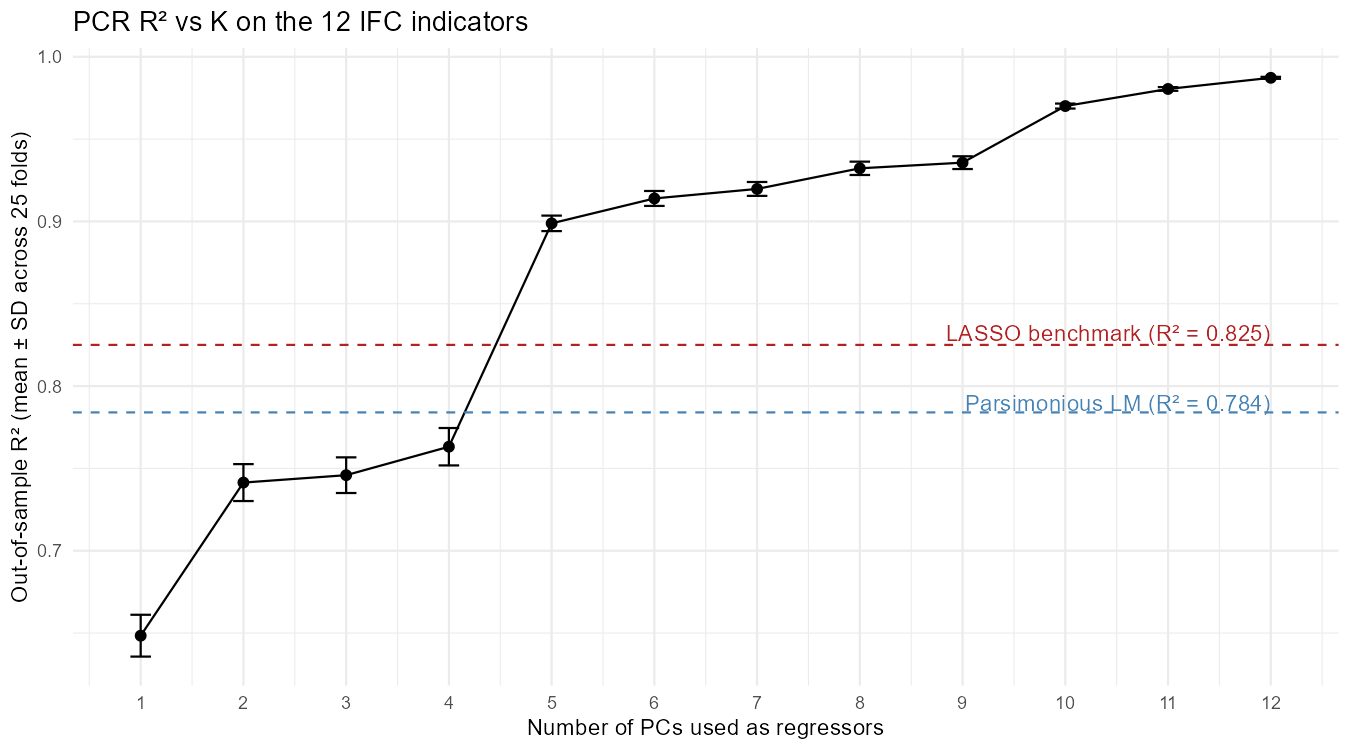
\includegraphics[width=0.85\textwidth]{figures/tradeoff_ifc.png}
  \caption{Curva di trade-off PCR sui 12 indicatori IFC. I due
    salti visibili, tra \(K = 4\) e \(K = 5\) e tra \(K = 9\) e
    \(K = 10\), sono la firma empirica della debolezza principale
    della PCR: la direzione predittiva non si allinea con le
    direzioni principali, quindi alcune PC "minori" portano una
    quota sproporzionata del contenuto predittivo per l'IFC.}
  \label{fig:trade_ifc}
\end{figure}

\paragraph{Un'illustrazione pulita del perché la PCR sbaglia il ranking.}
A \(K = 4\) la PCR ha usato il \(60\%\) della varianza di
\(\mathbf{X}\) ma raggiunge solo \(R^{2} = 0{,}763\). Aggiungendo
PC5 porta solo \(+7\%\) di varianza ma \(+0{,}14\) di \(R^{2}\).
La quinta direzione principale è quindi molto più informativa per
l'IFC di quanto la sua quota di varianza suggerirebbe. Lo stesso
è vero per PC10, con una discontinuità simile. È il motivo pratico
per cui la PLS, che usa \(y\) per ordinare le sue componenti, è il
metodo corretto per questo tipo di problema.

\subsection{Confronto diretto: la PLS domina la PCR}

Lo script 18c esegue PCR e PLS sulla stessa matrice GRINS a 326
feature e agli stessi valori di \(K\).
Tabella~\ref{tab:plspcr} e Figura~\ref{fig:plspcr} riportano il
risultato.

\begin{table}[h!]
  \centering
  \begin{tabular}{ccc c}
    \toprule
    \(K\) & PCR \(R^{2}\) & PLS \(R^{2}\) & gap PLS \(-\) PCR \\
    \midrule
    5    & 0,739 & 0,796 & \(+0{,}058\) \\
    10   & 0,761 & 0,810 & \(+0{,}049\) \\
    15   & 0,766 & 0,817 & \(+0{,}051\) \\
    20   & 0,769 & 0,820 & \(+0{,}051\) \\
    25   & 0,772 & \textbf{0,822} & \(+0{,}050\) \\
    30   & 0,776 & 0,823 & \(+0{,}047\) \\
    50   & 0,779 & 0,824 & \(+0{,}045\) \\
    75   & 0,780 & \textbf{0,825} & \(+0{,}045\) \\
    100  & 0,787 & 0,824 & \(+0{,}037\) \\
    \bottomrule
  \end{tabular}
  \caption{PCR vs PLS sulla matrice GRINS a 326 feature, CV
    panel-aware a 5 fold. La PLS domina la PCR di circa cinque
    punti di \(R^{2}\) a ogni \(K\). La PLS a \(K = 25\) batte
    già sia il modello lineare parsimonioso sia l'estensione
    mixed-model; la PLS a \(K = 75\) pareggia il benchmark LASSO.}
  \label{tab:plspcr}
\end{table}

\begin{figure}[h!]
  \centering
  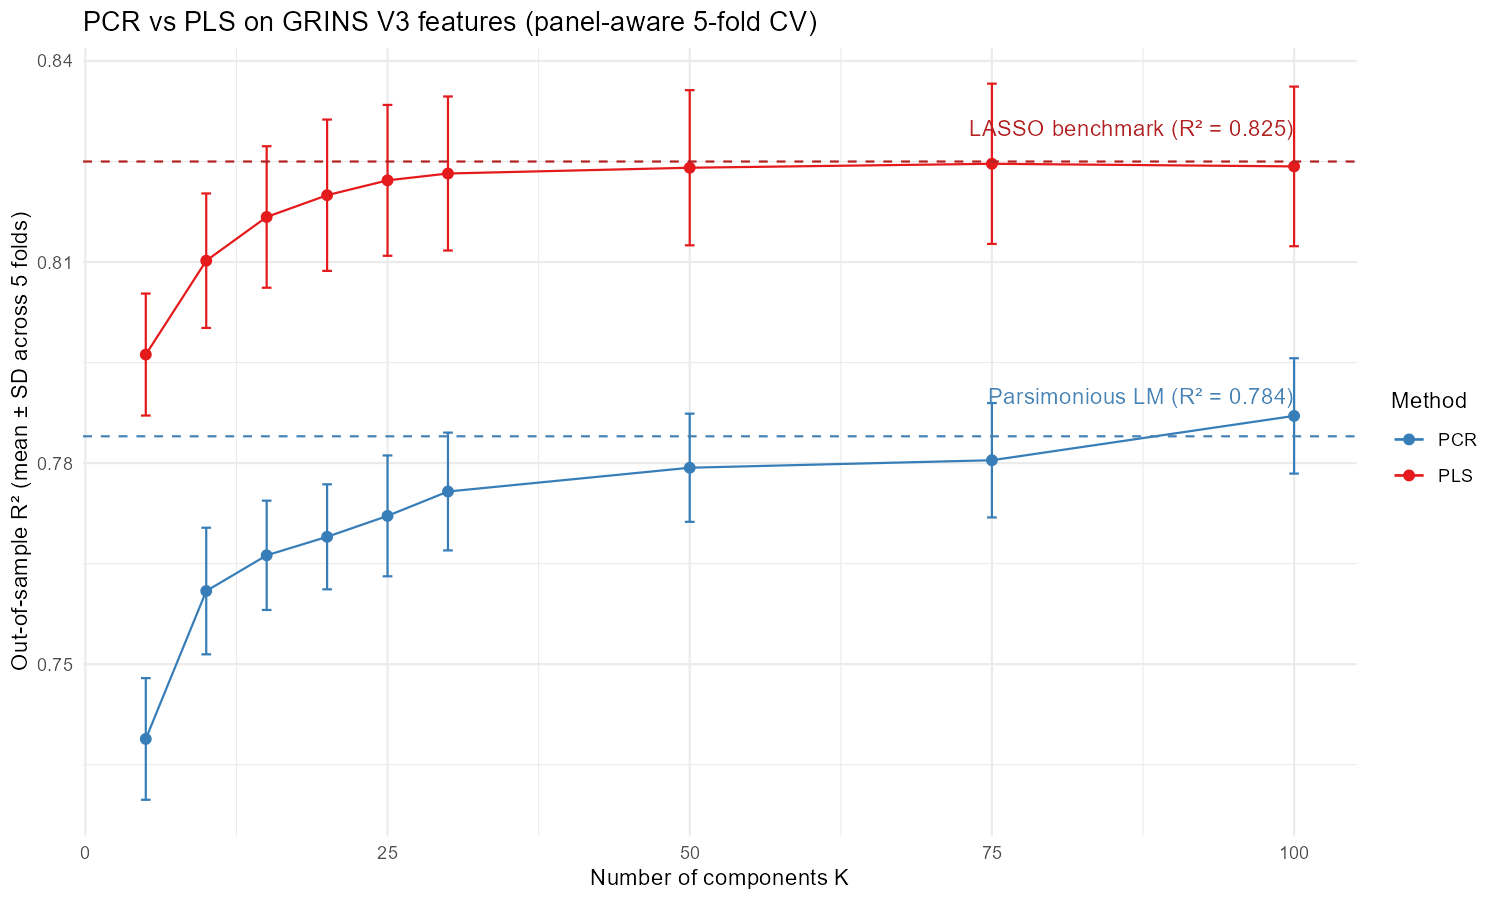
\includegraphics[width=0.95\textwidth]{figures/pls_vs_pcr.png}
  \caption{PLS vs PCR sulle feature GRINS V3. \(R^{2}\)
    out-of-sample su 5 fold di CV panel-aware, media \(\pm 1\)
    deviazione standard. La linea rossa tratteggiata è il
    benchmark LASSO; la linea blu tratteggiata è il modello
    lineare parsimonioso. La PLS raggiunge il benchmark LASSO a
    \(K \approx 75\); la PCR non lo raggiunge mai nel range
    esplorato.}
  \label{fig:plspcr}
\end{figure}

\paragraph{Tre osservazioni.}
Primo: il gap PLS--PCR è stabile e sostanziale: circa cinque punti
percentuali di \(R^{2}\) su tutto il range di \(K\). È molto più
grande della deviazione standard tra fold (\(\sim 0{,}01\)) e
quindi non è un artefatto di uno split favorevole. Secondo: la
PLS a \(K = 25\) fa già \(0{,}822\), che è meglio sia del modello
lineare parsimonioso a parità di complessità nominale (25
dimensioni) sia dell'estensione mixed-model
\(M_{\mathrm{geo,nested}}\). La PLS in questo senso è un upper
bound non-interpretabile sulla classe dei modelli lineari. Terzo:
la PLS si stabilizza intorno a \(K = 75\) a \(0{,}825\),
sostanzialmente in pari col benchmark LASSO a 191 covariate. I due
metodi raggiungono lo stesso tetto predittivo per strade diverse:
LASSO seleziona, PLS combina.

\section{Confronto con il resto del progetto}

La Tabella~\ref{tab:all} aggrega tutti i modelli stimati fino a
ora. La PLS a \(K=25\) e l'LMM \(M_{\mathrm{geo,nested}}\) a 25
covariate sono sostanzialmente in pari, e solo marginalmente sotto
il benchmark LASSO e la PLS a \(K=75\). La PCR è
sistematicamente sotto questo gruppo.

\begin{table}[h!]
  \centering
  \begin{tabular}{l c c l}
    \toprule
    Modello & dimensioni & \(R^{2}\) CV & interpretabilità \\
    \midrule
    Benchmark LASSO              & 191 var.\ GRINS & 0,826 & alta (variabili nominate) \\
    PLS su GRINS \((K = 75)\)    & 75 componenti   & 0,825 & bassa (variabili mixate) \\
    PLS su GRINS \((K = 25)\)    & 25 componenti   & 0,822 & bassa \\
    LMM \(M_{\mathrm{geo,nested}}\) & 25 var.\ + RE & 0,818 & alta \\
    PCR su GRINS \((K = 100)\)   & 100 componenti  & 0,787 & bassa \\
    LM parsimonioso              & 25 var.\ GRINS  & 0,784 & alta \\
    PCR su GRINS \((K = 25)\)    & 25 componenti   & 0,772 & bassa \\
    PCR su 12 IFC \((K = 12)\)   & 12 componenti   & 0,987 & quasi-tautologico \\
    \bottomrule
  \end{tabular}
  \caption{Tutti i modelli considerati nel progetto finora,
    ordinati per \(R^{2}\) out-of-sample all'interno del gruppo
    GRINS. L'ultima riga è inclusa solo per l'interpretazione
    diagnostica (PCR sui suoi stessi indicatori di input dell'IFC).}
  \label{tab:all}
\end{table}

\section{Conclusioni}

La richiesta del docente di estendere la PCA descrittiva in una
Principal Component Regression ha prodotto un insieme coerente di
findings metodologici.

\paragraph{La PCR sottoperforma perché varianza e predizione non si allineano.}
Sia sulla matrice GRINS a 326 feature sia sulla matrice
12-indicatori IFC, la PCR deve usare componenti molto più giù nel
ranking rispetto alle direzioni principali per catturare il
segnale IFC. L'esempio più chiaro è il salto di \(+0{,}14\) di
\(R^{2}\) a \(K = 5\) in Figura~\ref{fig:trade_ifc}: la PC5 porta
il 7\% della varianza di \(\mathbf{X}\) ma più contenuto predittivo
di PC1--PC4 messe insieme.

\paragraph{Il test di tautologia conferma che l'IFC non è pure-linear.}
La PCR sui 12 indicatori IFC si ferma a \(R^{2} = 0{,}987\), non a
\(1{,}0\). L'\(1{,}3\%\) restante non è rumore ma una
non-linearità strutturale nella costruzione dell'IFC (un passo di
rango percentuale o normalizzazione simile). È un utile controllo
di sanità sul target stesso.

\paragraph{La PLS aggiusta il disallineamento ma perde interpretabilità.}
La PLS, che usa \(y\) nella scelta delle componenti, domina la PCR
di circa cinque punti di \(R^{2}\) a ogni \(K\). La PLS a
\(K = 75\) pareggia il benchmark LASSO; la PLS a \(K = 25\) è
sostanzialmente in pari con il mixed model geografico annidato. Il
benchmark LASSO non è quindi un'accidente speciale della penalità:
qualsiasi proiezione lineare 75-dimensionale ben scelta delle
feature GRINS raggiunge lo stesso tetto predittivo. Quello che il
LASSO compra è l'\emph{interpretabilità}: 25 covariate nominate
con segni espliciti e effetti standardizzati, invece di 25 o 75
combinazioni lineari di tutte le 326 feature.

\paragraph{Take-away per il progetto.}
La pipeline LASSO + LMM mantiene il suo posto come deliverable
preferito. La PCR è documentata qui come controllo metodologico
(è ciò che si ottiene trattando la riduzione di dimensionalità
come sostituto della selezione di variabili), e la PLS è
documentata come il miglior upper bound lineare non-interpretabile.
La scelta tra LASSO e PLS a \(K = 75\) è essenzialmente una
scelta tra variabili interpretabili e un modello illeggibile ma
leggermente più grande: nel nostro contesto raggiungono la stessa
accuratezza predittiva.

\end{document}
